\chapter{EPDrawGUI}\label{epdrawgui}

The EPDrawGUI program is a simple utility that can be used to generate a dxf file from an input file without running EnergyPlus. It is a simple cross platform application is stored in the Preprocess subfolder of the EnergyPlus folder upon installation. A companion DLL (EPlusDrw.dll) is also needed in the same folder. And its library folders are required in a subfolder (EPDrawGUI Libs).

\begin{figure}[hbtp] % fig 30
\centering
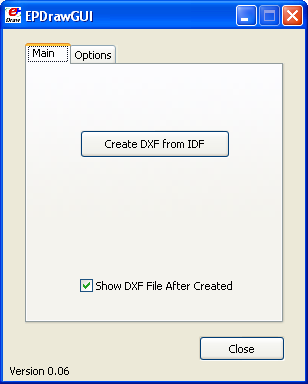
\includegraphics[width=0.9\textwidth, height=0.9\textheight, keepaspectratio=true]{media/image028.png}
\caption{EPDrawGUI Main Screen \protect \label{fig:epdrawgui-main-screen}}
\end{figure}

Help is offered on the Main Tab and on the Options Tab when you place the mouse, without clicking, over the buttons, check boxes, and option boxes. In addition, the program copyright information is displayed when the mouse is over the Version number text in the lower left corner.
